%%%%%%%%%%%%%%%%%%%%%%%%%%%%%%%%%%%%%%%%%
%
% CMPT 435
% Spring 2019
% Lab One
%
%%%%%%%%%%%%%%%%%%%%%%%%%%%%%%%%%%%%%%%%%

%%%%%%%%%%%%%%%%%%%%%%%%%%%%%%%%%%%%%%%%%
% Short Sectioned Assignment
% LaTeX Template
% Version 1.0 (5/5/12)
%
% This template has been downloaded from: http://www.LaTeXTemplates.com
% Original author: % Frits Wenneker (http://www.howtotex.com)
% License: CC BY-NC-SA 3.0 (http://creativecommons.org/licenses/by-nc-sa/3.0/)
% Modified by Alan G. Labouseur  - alan@labouseur.com
%
%%%%%%%%%%%%%%%%%%%%%%%%%%%%%%%%%%%%%%%%%

%----------------------------------------------------------------------------------------
%	PACKAGES AND OTHER DOCUMENT CONFIGURATIONS
%----------------------------------------------------------------------------------------

\documentclass[letterpaper, 10pt]{article} 


\usepackage[english]{babel} % English language/hyphenation
\usepackage[utf8]{inputenc}
\usepackage{graphicx}
\usepackage[lined,linesnumbered,commentsnumbered]{algorithm2e}
\usepackage{listings}
\usepackage{minted}
\usepackage{fancyhdr} % Custom headers and footers
\pagestyle{fancyplain} % Makes all pages in the document conform to the custom headers and footers
\usepackage[table]{xcolor}
\usepackage{csquotes}
\usepackage{natbib}
\usepackage[nottoc]{tocbibind}
\usepackage{lastpage}
\usepackage{url}
\usepackage{float}
\usepackage{scrextend}
\usepackage{epigraph}
\fancyhead{} % No page header - if you want one, create it in the same way as the footers below
\fancyfoot[L]{} % Empty left footer
\fancyfoot[C]{page \thepage\ of \pageref{LastPage}} % Page numbering for center footer
\fancyfoot[R]{}
\usepackage{listings}% http://ctan.org/pkg/listings
\usepackage{hyperref}
\renewcommand{\headrulewidth}{0pt} % Remove header underlines
\renewcommand{\footrulewidth}{0pt} % Remove footer underlines
\setlength{\headheight}{13.6pt} % Customize the height of the header
\usepackage{pgfplots}

\pgfplotsset{width=7cm,compat=1.8}

%----------------------------------------------------------------------------------------
%	TITLE SECTION
%----------------------------------------------------------------------------------------

\newcommand{\horrule}[1]{\rule{\linewidth}{#1}} % Create horizontal rule command with 1 argument of height

\title{	
   \normalfont \normalsize 
   \textsc{CMPT 435 - Fall 2020 - Dr. Labouseur} \\[10pt] % Header stuff.
   \horrule{0.5pt} \\[0.25cm] 	% Top horizontal rule
   \large{Assignment Five -- Bellman-Ford, Spice, and Everything Nice} \\
   \textsc{Bellman-Ford Single Source Shortest Path Algorithm, and a Greedy Solution to the Fractional Knapsack Problem}\\[20pt]% Assignment title
 \author{Sam Alcosser \\ \normalsize Samuel.Alcosser1@Marist.edu}
   \horrule{0.5pt} \\ 	% Bottom horizontal rule
   


	% Today's date.
  
\date{\normalsize\today} 
}
\begin{document}




\fontfamily{bch}\selectfont
\maketitle
\tableofcontents
\newpage

\section{Introduction}

For this documentation, there is a different format for how the processes are displayed. in this new format, the layout of each process will be outlined in an explanation, then all of the necessary data structures will be explained, and finally a step by step breakdown of the process itself will be given with direct references to line numbers. 

To improve the flow of the document itself, smaller pieces such as header files, data structures, and supplementary methods will have outlines of their actual code in the appendix. This way, the reader can read at their own pace, depending on their level of prior knowledge of the topic.



\section{Bellman-Ford Single Source Shortest Path (SSSP)}
\begin{center}
 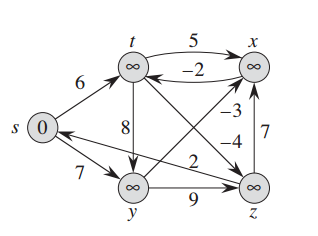
\includegraphics[width=\textwidth / 2 ]{Bellman-Ford-Algorithm-1.png}
 \end{center}
 
This algorithm works on weighted graphs. Weighted graphs are sets of vertices with one-way paths going between them, and each path, or edge, is assigned a weight. Although, not all vertices must be connected to each vertex, and edges can have negative weights. Also, all of the vertices hold a distance value which will be discussed later (For more explanation, see the Appendix for code explanations of vertices and edges) .

The Bellman-Ford SSSP algorithm, and single source shortest path algorithms in general, exactly what they sound like. They are ways to find the least costly and "shortest path" from a "single source" vertex to any of the other vertices in the graph. Bellman-Ford is a SSSP algorithm that is also useful as it can indicate whether or not there is a negative weight cycle. The process works in three main steps.
\begin{enumerate}
    \item Start with all but the first vertex having a distance of $\infty$, as the first "source" vertex will be set to a distance of 0.
    \item "Relax", or update, the distances of the vertices using the weights of each edge. Repeat the updating process a number of times equivalent to the number of vertices in the graph to ensure the distances are correct.
    \item Check for negative weight cycles by iterating over each edge one more time. If a negative weight cycle is found, return as false, otherwise, continue in order to return true.
\end{enumerate}

Thankfully, the implementation of this code more or less is broken up by those three steps. To begin , there is the \texttt{init()} function.
\vspace{.5em}

\textbf{Note:} For a detailed explanation of how the data actually gets into the graph at the beginning, see the Appendix for the description of method \texttt{fileReader()}


\subsection{\texttt{GraphManager::init()}: Initializing the Vertices}

This first part of the algorithm is simply used to set up the initial distances of the vertices (hence the name \texttt{init()}).


 \begin{addmargin}[-5em]{1em}
\begin{small}
\begin{minted}[linenos=true]{cpp}
void GraphManager::init(Vertex *source)
{
	for (int i = 0; i < graph.size(); i++)
	{
		graph[i]->distance = 10000000;
		graph[i]->prev = nullptr;
	}
	source->distance = 0;

}
\end{minted}
\end{small}
\end{addmargin}

The process in this function is very simple to see. It iterates a number of times equivilent to the size,  or more specifically cardinality, of the graph's vertices(line 3). For each iteration it sets the indexed vertex to have a distance of 10000000, and a \texttt{nullptr} for its previous vertex (lines 5-6). The reason for the use of the number 10,000,000 and not infinity is that support of a real infinite value in C++ is very hit or miss. 

When implementing one package which defines a global constant called \texttt{INIFINITY}, a quick printout shows that the values are so large that they seem to have rolled over into  incredibly large negative numbers. So, after seeing that the real function of this value was to be a placeholder value that would undoubtedly be greater than any weight that could be defined, ten million was decided to be a safe value to imitate infinity. Finally, the source vertex is set to a distance of 0 (line 8).



\subsection{\texttt{GraphManager::relax()}: Updating Distances Using the Edges}

The second key aspect of this algorithm is the process of "relaxing" edges.

 \begin{addmargin}[-5em]{1em}
\begin{small}
\begin{minted}[linenos=true]{cpp}
void GraphManager::relax(Edge *edge, Vertex *from, Vertex *dest)
{
	if (dest->distance > from->distance + edge->weight)
	{
		dest->distance = from->distance + edge->weight;
		dest->prev = from;
	}
}
\end{minted}
\end{small}
\end{addmargin}      
This process will take an edge and its two related vertices and attempt to update the destination vertex. The vertex will only be changed if the destination vertex's distance is greater than the sum of the distance of the \texttt{from} vertex and the \texttt{weight} of the edge combined (line 3). If this is the case,  the distance of the destination vertex will be updated to that previously described sum, and it's previous vertex pointer will take the address of the from vertex (lines 5-6). 

Realistically, it would've been possible to only pass the edge itself to this method. Although, within the process, it would have made for much dirtier code. There would need to be long chains of pointers to class members in many places. Therefore, all three parts are passed.

\subsection{\texttt{GraphManager::Bellman()} : Bringing it All Together}

Since the sub parts of this algorithm have been previously described, the algorithm itself should now make sense
 \begin{addmargin}[-5em]{1em}
\begin{small}
\begin{minted}[linenos=true]{cpp}
bool GraphManager::Bellman()
{
	init(graph[0]);
	for (int i = 0; i < graph.size(); i++)
	{
		for (Edge *e : weightMatrix)
		{
			relax(e, e->from, e->dest);
		}
	}
	for (int q = 0; q < weightMatrix.size(); q++)
	{
		if (weightMatrix[q]->dest->distance > weightMatrix[q]->from->distance + weightMatrix[q]->weight)
		{
			cout << "Uh Oh! Found a negative cycle!" << endl;
			return false;
		}
	}

	for (int n = 1; n < graph.size(); n++)
	{
		printPath(graph[0], graph[n]);
	}

	return true;
}

\end{minted}
\end{small}
\end{addmargin}   


\begin{itemize}
    \item Part 1 (line 3): initialize the graph with the \texttt{init()} method.
    \item Part 2 (lines 4-10): Relax using each edge using the \texttt{relax()} method a number of times equivalent to the cardinality of the set of vertices.
    \item Part 3 (lines 11-18): Test each edge for negative cycles. if the distance of the destination vertex is greater than the sum of the distance of the \texttt{from} vertex and the weight of the edge combined, report a negative cycle and return \texttt{false}.
    \item Part 4 (lines 20-23): For every non-source vertex, print the path from the source to that vertex using the \texttt{printPath()} method (described in detail in the appendix).
    \item Part 5 (line 25): Since the function would have been returned by this point if there was a negative cycle, we can assume that there are shortest paths to every point, so we return true.
\end{itemize}

\subsection{Asymptotic Analysis of Bellman-Ford SSSP}

This algorithm completes in $O(VE)$ time. The reason being that the initialization process takes $O(V)$ time,  the relaxing process is completed $E$ times for every  vertex in $V$, and the final check runs $E$ times. Before accounting for constants and unnecessary numbers, this would seem like $O(2V*2E)$, although once simplified it becomes $O(VE)$.

\section{Greedy Algorithms and Fractional Knapsack}

Dynamic programming is a way of finding the best approach to solving a problem, and using the optimal solution. A very simple version of this is the greedy algorithm that can be used for the fractional knapsack problem. Say that there are multiple different spices, each in a different amount, and a different cost per unit. You want to fit as much value, in spice, as you can into your knapsack of finite capacity. The greedy algorithmic approach to this would have you do a defined set of steps.

\begin{enumerate}
    \item Find the unit price of each of the spices by dividing their total price by their quantity.
    \item Sort the spices in order from most expensive per unit to least expensive per unit.
    \item Starting with the most expensive spice, take as much as you can of that spice. If not all will fit, take whatever fraction will fit in the knapsack. Continue until the knapsack is full.
\end{enumerate}

\subsection{\texttt{Greedy::greedyAlgo()}: Filling the Knapsacks}

This method is called by the method which reads in the input file whenever a new knapsack capacity is given. This means that by this point in the processing, all of the spices have been inputted, their individual unit prices have been calculated, and they have been sorted from least to greatest using Merge Sort (more on this later). With all of this set up, the stealing of the spices can commence.



 \begin{addmargin}[-5em]{1em}
\begin{small}
\begin{minted}[linenos=true]{cpp}
void Greedy::greedyAlgo(int capacity)
{

    struct Portion
    {
        double qty;
        Spice *spice;
    };

    int cTotal = 0;
    vector<Portion *> ks;
    double earnings = 0;
    while (cTotal != capacity)
    {
        
        for (int i = spices.size() - 1; i > 0; i--)
        {
            if ((cTotal + spices[i]->qty) <= capacity)
            {

                Portion *p = new Portion();
                p->qty = spices[i]->qty;
                p->spice = spices[i];
                cTotal += spices[i]->qty;
                ks.push_back(p);
                earnings += p->spice->tPrice;
            }
            else if (((capacity - cTotal) > 0) && ((cTotal + spices[i]->qty) > capacity))
            {

                Portion *part = new Portion();
                part->qty = capacity - cTotal;
                part->spice = spices[i];
                cTotal += part->qty;
                ks.push_back(part);
                earnings += ((part->spice->uPrice) * (part->qty));
                break;
            }
        }
    }
    ...
    // printout code not integral to algorithm
    ...
}
\end{minted}
\end{small}
\end{addmargin}   

Two things must be discussed before explaining the code above. First of all, there is the \texttt{struct} called \texttt{Portion} that was used to handle the data for each portion of the spices which is defined to be used in this function. This structure will hold the quantity of that spice that is being taken, and the spice itself. Second, there is the prospective issue of not sorting from greatest to least. On line 16, it is seen that my iterator variable \texttt{i} is counting down from the last index of the spice list to the first. With this little tweak, my array of spices can be read in the same way, and with the same complexity as it is still using merge sort, and it is still iterating the same number of times only in reverse. Now, on to the process. 

\begin{enumerate}
    \item Start the current load counter \texttt{cTotal} and the \texttt{earnings} variables to 0, and initialize the vector to hold \texttt{Portion} structs and call it \texttt{ks}(lines 10-13).
    \item Continue the following process until the \texttt{cTotal} variable matches the \texttt{capacity} of the knapsack, as passed in to the method (line 13).
    \item Iterate over the list of sorted spices from greatest to smallest by iterating in reverse (line 16).
    \item Check if the whole amount of the spice could fit in the knapsack (line 18)
        \begin{itemize}
            \item If it can, add the whole spice as a portion to the \texttt{ks} vector with its quantity and the spice itself (lines 21-23, 25). Next update the \texttt{cTotal} with the new volume, and the total price of the spice (lines 24,26).
            \item If it cannot, add an amount equivalent to the remaining space in the knapsack (lines 31-33, 35). Finally, update the \texttt{cTotal} and the \texttt{earnings} variables(34,36). Break out of the for loop (line 37).
        \end{itemize}

\end{enumerate}

\subsection{Asymptotic Analysis of The Greedy Algorithm for Fractional Knapsack}

Fractional knapsack runs in $O(n \lg{n})$ time. The reason being that in the beginning, the process will just iterate until it cannot fit whole spice piles into its knapsack ($n$), but as it gets closer to filled there are fewer and fewer things that can be fit into the knapsack ($\lg{n}$).


\newpage


\section{Appendix}

\subsection{Bellman-Ford SSSP Extras}
\subsubsection{Header Files}

\textbf{GraphManager.h : The Graph Class}
 \begin{addmargin}[-5em]{1em}
\begin{small}
\begin{minted}[linenos=true]{cpp}
#pragma once
#include <iostream>
#include <string>
#include <vector>
#include "Vertex.h"
#include "Edge.h"
using namespace std;
class GraphManager{
    public:
    vector<Vertex*> graph;
    vector<Edge *> weightMatrix;
    void fileReader(string fileName);
    void init(Vertex * source);
    void relax(Edge * edge, Vertex * from, Vertex * dest);
     bool Bellman();
     void printPath(Vertex * source, Vertex * dest);
};

\end{minted}
\end{small}
\end{addmargin}   

\begin{itemize}
    \item \texttt{graph} and \texttt{weightMatrix} hold the vertices and edges respectivley
    \item \texttt{fileReader()} is used to read the file and also run the algorithm
    \item \texttt{init()} is used to initialize the graph
    \item \texttt{relax()} is used to  relax the edges of the graph
    \item \texttt{Bellman()} is the method used to carry out the process of the algorithm
    \item \texttt{printPath()} is used to print the paths from the source vertex to each of the other vertices
\end{itemize}


\textbf{Edge.h : Edges of the Weighted Graph}
 \begin{addmargin}[-5em]{1em}
\begin{small}
\begin{minted}[linenos=true]{cpp}
#pragma once
#include <iostream>
#include "Vertex.h"
class Vertex;
class Edge
{
public:
    int weight;
    Vertex *dest;
    Vertex *from;
};

\end{minted}
\end{small}
\end{addmargin}   

\begin{itemize}
    \item \texttt{weight} holds the weight of the edge
    \item \texttt{*dest} holds a pointer to the destination vertex of the edge
    \item \texttt{*from} holds a pointer to the origin vertex of the edge
\end{itemize}


\textbf{Vertex.h : Vertices of the Weighted Graph}
 \begin{addmargin}[-5em]{1em}
\begin{small}
\begin{minted}[linenos=true]{cpp}
#pragma once
#include <iostream>
#include <vector>
#include "Edge.h"
class Edge;
class Vertex
{
public:
    int id;
    int distance;
    Vertex *prev;
};

\end{minted}
\end{small}
\end{addmargin}   

\begin{itemize}
    \item \texttt{id} holds the id of the vertex so it can be identified later
    \item \texttt{distance} holds a the distance to a given vertex from the source vertex
    \item \texttt{*prev} holds a pointer to the vertex directly before
\end{itemize}

\subsubsection{Helper Methods}

\textbf{\texttt{GraphManager::fileReader()}  : Reading in the Input File}
 \begin{addmargin}[-5em]{1em}
\begin{small}
\begin{minted}[linenos=true]{cpp}
void GraphManager::fileReader(std::string fileName)
{

	fstream newfile;

	string ln;
	int count = 0;
	bool started = false;
	newfile.open(fileName, ios::in);
	if (newfile.is_open())
	{
		while (getline(newfile, ln)) 
		{

			if (ln.find("new graph") != string::npos)
			{

				if (started)
				{
cout << "**********************************"<<endl;
					Bellman();

					weightMatrix.clear();
					graph.clear(); //restarting the graph
				}
				started = true;
			}
			else if (ln.find("add vertex") != string::npos)
			{
				int id = stoi(ln.substr(11));
				Vertex *vertex = new Vertex();
				vertex->id = id;
				graph.push_back(vertex); 
			}
			else if (ln.find("add edge") != string::npos)
			{

				int hyph = ln.find("-");

				int num1 = stoi(ln.substr((ln.find("edge") + 5), 2)); 
				int num2 = stoi(ln.substr(hyph + 2, 2));
				int weight = stoi(ln.substr(hyph + 4));
				
				for (int i = 0; i < graph.size(); i++) 
				{
					if (graph[i]->id == num1)
					{
						for (int j = 0; j < graph.size(); j++)
						{
							if (graph[j]->id == num2)
							{

								Edge *e = new Edge();
								e->weight = weight;
								e->dest = graph[j];
								e->from = graph[i];
							
								weightMatrix.push_back(e);
							
							}
						}
					}
				}
			}
		}
	}
	newfile.close();
	cout << "**********************************"<<endl;
	Bellman();
	return;
};

\end{minted}
\end{small}
\end{addmargin}   
\begin{enumerate}
    \item If somewhere in the line it says "add vertex", assume this means it is defining a vertex. Grab the integer id from the assumed position in the string, and assign it to the \texttt{id} of a new vertex before adding it to the graph(lines 28-34)
    \item If the line says "add edge" pull out the ids of both of the defined vertices, and the weight (lines 35-42). Using two "fingers" from nested for loops, find the two verticies in the graph, make them into the \texttt{from} and \texttt{dest} on a new edge, add the weight, and push the edge back on to the list of edges (lines 35-68)
    \item If the line says new graph, we can assume that all of the information for the previous graph has been given. Although, if this is the first time seeing New Graph, this could just be the beginning of the file. So, if it is the first time simply raise the \texttt{started} flag and continue. Otherwise, run \texttt{Bellman()}, and then clear the graphs vertices and edges.(lines 15-27)
    \item Since "new graph" only occurs before a new graph, we need to run \texttt{Bellman()} once more at the end to process the final data points (line 68).
\end{enumerate}

\textbf{\texttt{GraphManager::printPath()} : Printing the Paths From The Source }
 \begin{addmargin}[-5em]{1em}
\begin{small}
\begin{minted}[linenos=true]{cpp}
void GraphManager::printPath(Vertex *source, Vertex *dest)
{
	vector<Vertex *> traceback;
	cout << source->id << "->" << dest->id << " cost is " << dest->distance << "; path: ";
	bool found = false;
	Vertex *currentV = dest;
	while (!found)
	{
		if (currentV->id != source->id)
		{
			
			traceback.push_back(currentV);
			currentV = currentV->prev;
		}
		else
		{
			
			found = true;
		}
	}
	cout << source->id;

	for (int i = traceback.size() - 1; i >= 0; i--)
	{
		cout << "->" << traceback[i]->id;
	}
	cout << endl;
}

\end{minted}
\end{small}
\end{addmargin}   

\begin{enumerate}
    \item Start by printing out the cost of the path by taking the \texttt{distance} of the \texttt{dest} vertex (line 4).
    \item Make a placeholder \texttt{Vertex} pointer at the destination vertex that was passed to the method, and make a \texttt{vector} to hold the vertices that are found on the trace back through the path (lines 3, 6).
    \item Starting with our placeholder at the destination, add our placeholder vertex to the traceback, and set the new placeholder to the previous vertex of our placeholder vertex (lines 12,13). Continue this process until the placeholder vertex \texttt{currentV} matches our \texttt{source} vertex (lines 7-20)
    \item Starting from the back, print out the id of each of the vertices in the \texttt{traceback} \texttt{vector} (lines 23-27).
\end{enumerate}

\subsection{Fractional Knapsack Extras}
\subsubsection{Header Files}

\textbf{Greedy.h : The Knapsack Class}
 \begin{addmargin}[-5em]{1em}
\begin{small}
\begin{minted}[linenos=true]{cpp}
#pragma once
#include <string>
#include <vector>
#include "Spice.h"
using namespace std;
class Greedy
{
public:
    void setupSpices(std::string fileName);
    void greedyAlgo(int capacity);
    vector<Spice *> spices;
};


\end{minted}
\end{small}
\end{addmargin}   

\begin{itemize}
    \item \texttt{setupSpices()} reads the input file and runs the algorithm
    \item \texttt{greedyAlgo()} runs a greedy algorithm for the Fractional Knapsack problem
    \item \texttt{spices} holds a list of spices
\end{itemize}

\textbf{Spice.h : The Spice Data Structure}
 \begin{addmargin}[-5em]{1em}
\begin{small}
\begin{minted}[linenos=true]{cpp}
#pragma once
#include <string>

class Spice{
    public:
    std::string color;
    double tPrice;
    int qty;
    int uPrice;


    void setPrice(double tPrice, double qty){
        this->tPrice = tPrice;
        this->qty = qty;
        this->uPrice = tPrice / qty;
        
    }
};

\end{minted}
\end{small}
\end{addmargin}   

\begin{itemize}
    \item \texttt{color} is used to identify the spice
    \item \texttt{tPrice} holds the total price of the spice
    \item \texttt{qty} holds the quantity of the spice
    \item \texttt{uPrice} holds the unit price for the spice
    \item \texttt{setPrice()} takes both the total price and the quantity in, and sets the values for the total price, quantity, and the unit price by dividing the total price by the quantity
\end{itemize}

\subsubsection{Helper Methods}

\textbf{\texttt{Greedy::setupSpices()} : Setup for Spices and Running the Algorithm}
 \begin{addmargin}[-5em]{1em}
\begin{small}
\begin{minted}[linenos=true]{cpp}
void Greedy::setupSpices(std::string fileName)
{

    fstream newfile;

    string ln;

    bool sorted = false;
    newfile.open(fileName, ios::in);
    if (newfile.is_open())
    {
        while (getline(newfile, ln)) //read each line of the file
        {

            if (ln.find("knapsack capacity") != string::npos)
            {

                if (!sorted)
                {
                    //sort the stuff
                    Sort::mergeSort(spices, 0, spices.size() - 1);
                    sorted = true;
                }
                int cap = stoi(ln.substr(19, 3));

                cout << "**********************************" << endl;
                greedyAlgo(cap);
                cout << "**********************************" << endl;
            }
            else if (ln.find("spice name") != string::npos)
            {
                vector<string> parts;

                for (int i = 0; i < ln.size(); i++)
                {
                    if (ln[i] == ';')
                    {
                        for (int j = (i - 1); j > 0; j--)
                        {
                            if (ln[j] == '=')
                            {

                                string sub = ln.substr(j + 2, (i - j) - 2);

                                parts.push_back(sub);
                                
                                break;
                            }
                        }
                    }
                }

                Spice *nSpice = new Spice();
                nSpice->color = parts[0];
                nSpice->setPrice(stod(parts[1]), stod(parts[2]));
                spices.push_back(nSpice);

               
            }
        }
    }
    newfile.close();

    return;
};
\end{minted}
\end{small}
\end{addmargin}   



\begin{enumerate}
    \item If the current line contains "spice name", we can assume that this is the data for a spice. Because we know that the three data points for the spice always occur between an "=" and a ";", and each of the three data points always occur in the same order, we can systematically find each point. We will keep these points in a string vector called \texttt{parts}.(line 30)
    \item Whenever the outer for loop has its index on a semicolon(line 36), back track from this index until a "=" is found (38-40).
    \item Take the substring of the line using the two indexes \texttt{i} and \texttt{j}, adjusting slightly to mitigate white space. Then, add this substring to \texttt{parts}. Break the inner loop to continue searching for the next data point's semicolon(lines 43-47).
    \item Make a new spice object, using the first item in \texttt{parts} as the color, and using the second and third items as the total price and quantity. This is applied using the \texttt{Spice::setPrice()} function which was described previously. Once created, add it to the list of spices (lines 53-56).
    \item If the line contains "knapsack capacity", we can assume that this is giving the capacity of a knapsack. Therefore we know that all of the spices have been given and we can begin filling our knapsack. (line 15)
    \item If this is the first time the algorithm is running, as denoted by the \texttt{started} flag not being set, then run merge sort on the spices to sort them from least expensive to most expensive by unit price. This sort is largely unchanged thanks to the ability to access items from a vector in a similar way to arrays. Other than changes to signatures, and changing to comparing the spices unit prices, nothing has been changed from previous uses of this sort.(lines 18-23)
    \item After this process has been ran, or skipped, grab the correct substring of the line and turn it into an integer. This will be the capacity of the knapsack. Finally run the \texttt{greedyAlgo()} function with the correct capacity for the knapsack. (lines 24-27)
\end{enumerate}


\textbf{\texttt{Greedy::greedyAlgo()} : The Output Functionality}

This section was added in the appendix as it was unneeded in the main portion of the document to convey the process of the algorithm. By this point, the knapsack is filled and all that is left is to print out what we escaped with.

 \begin{addmargin}[-5em]{1em}
\begin{small}
\begin{minted}[linenos=true]{cpp}
void Greedy::greedyAlgo(int capacity)
{

...
...//Actual Algorithm Code
...

    cout << "Knapsack of capacity " << capacity << " is worth " << earnings << " quatloos and" << endl;
    cout << "contains ";
    for (int n = 0; n < ks.size(); n++)
    {

        if (n == 0)
        {
            if (ks[n]->qty == 1)
            {
                cout << ks[n]->qty << " scoop of " << ks[n]->spice->color;
            }
            else
            {
                cout << ks[n]->qty << " scoops of " << ks[n]->spice->color;
            }
        }
        else
        {
            if (ks[n]->qty == 1)
            {
                cout << ", " << ks[n]->qty << " scoop of " << ks[n]->spice->color;
            }
            else
            {
                cout << ", " << ks[n]->qty << " scoops of " << ks[n]->spice->color;
            }
        }
    }
    cout << "." << endl;
}

\end{minted}
\end{small}
\end{addmargin}   


\begin{enumerate}
    \item Print out an opening line containing the total \texttt{earnings} from the knapsack (line 8)
    \item For each \texttt{Portion} in the knapsack, list it's quantity followed by its color. Adjust grammar based on the quantity and whether or not it is the first item in the list. Meaning, adding an "s" to "scoop" for quantities greater than 1, and adding a comma before the statement if it is not the first item (lines 10-35)
    \item Don't forget the period. (line 36)
\end{enumerate}


\subsection{Extras}
\textbf{Main.cpp : Putting Everything Together}
 \begin{addmargin}[-5em]{1em}
\begin{small}
\begin{minted}[linenos=true]{cpp}

#include <iostream>
#include <string>
#include "GraphManager.h"
#include "Greedy.h"
using namespace std;

int main()
{

	GraphManager *gm = new GraphManager();
	gm->fileReader("graphs2.txt");
	Greedy * greed = new Greedy();
	greed->setupSpices("spice.txt");
	return 0;
}
\end{minted}
\end{small}
\end{addmargin}   

\begin{enumerate}
    \item Setup and run the \texttt{GraphManager} for Bellman-Ford SSSP with the "graphs2.txt" file (lines 10,11)
    \item Setup and run the \texttt{Greedy} object for fractional knapsack using the input file "spice.txt" (lines 12,13)
\end{enumerate}

\textbf{References}

8, Manan Soni May. “Bellman-Ford Algorithm in C and C++.” The Crazy Programmer, 3 June 2017, www.thecrazyprogrammer.com/2017/06/bellman-ford-algorithm-in-c-and-c.html. 



\vspace{2.5em}

\subsection{Conclusion}
\textbf{Closing Thoughts}

As with all of the assignments this semester, we were tasked with implementing algorithms. This meant that once we understood the algorithm well enough, we were generally able to complete the project without having to "Solve" anything new. Other than some slight issues with the language that I ran into, or issues when it came to not completely understanding the algorithm. 

For this reason, I enjoyed this assignment as I was able to solve somewhat open ended problems like how to use an existing sorting algorithm without doing extra unnecessary work. Or even the way I devised to parse the input strings for the file. To me, these were the most satisfying problems to solve.

\vspace{1em}
\newline

as a wise person once said, "
give a person a program and they'll be
frustrated for a day, teach a person to
program and they'll be frustrated for the
rest of their life.".
 \vspace{.5em}
{\textit{\color{red}\huge{\{S.A.\}}}}

\vspace{1em}

\end{document}

